
\section{The Frequency Response}


%\begin{frame}
%\frametitle{The transfer function}
%
%From previous lectures:
%\begin{align*}
%    y(t) &= h(t) \otimes u(t)  \\
%    \Rightarrow \quad 
%    \mathscr{L}\{y(t)\} &= \mathscr{L}\{h(t) \otimes u(t)\}  \\
%    \Rightarrow \quad
%    Y(s) &= H(s) \cdot U(s)\\
%    H(s) &= \frac{Y(s)}{U(s)}
%\end{align*}
%This is the transfer function, the relation between input and output in the Laplace domain (continuous time systems)
%
%
%\end{frame}
%
%\begin{frame}
%\frametitle{Plot of H(s)?}
%
%\begin{itemize}
%\item $s$ and $H(s)$ are both complex $\rightarrow$ 4D-graph?
%\item No, we will substitute $s$ for $j\omega$ with $\omega$ the angular frequency [rad/s].
%(We will often use frequency to indicate $\omega$ but keep in mind that $\omega = 2\pi f)$
%\item We will also split $H(s) = H(j\omega)$ using its polar representation in two, an magnitude and a phase plot
%\item Remember: $H(j\omega) = |H(j\omega)| \exp\angle(H(j\omega))$ 
%\item The magnitude plot and the phase plot of $H(j\omega)$ are called the bode plot
%
%\end{itemize}
%\end{frame}


\begin{frame}
\frametitle{What is the frequency response of a system?}
\begin{definition}
	\begin{itemize}
		\item Frequency response = steady state response of a system to a sinusoidal input.\\
		\item Assume an input $x(t) = X\sin(\omega t)$.\\
		\item The output in a linear system is then also sinusoidal, with a change in the magnitude and phase, i.e. $y(t) = Y\sin(\omega t + \phi)$.\\
		\item It can be shown that: $Y = X\cdot |H(j\omega)|$ and $\phi = \angle H(j\omega)$.\\
		\item $H(j\omega)$ is therefore also called the sinusoidal transfer function. 
	\end{itemize}
\end{definition}




\end{frame}

\begin{frame}
\frametitle{Relation of sinusoidal input/output in a linear system}


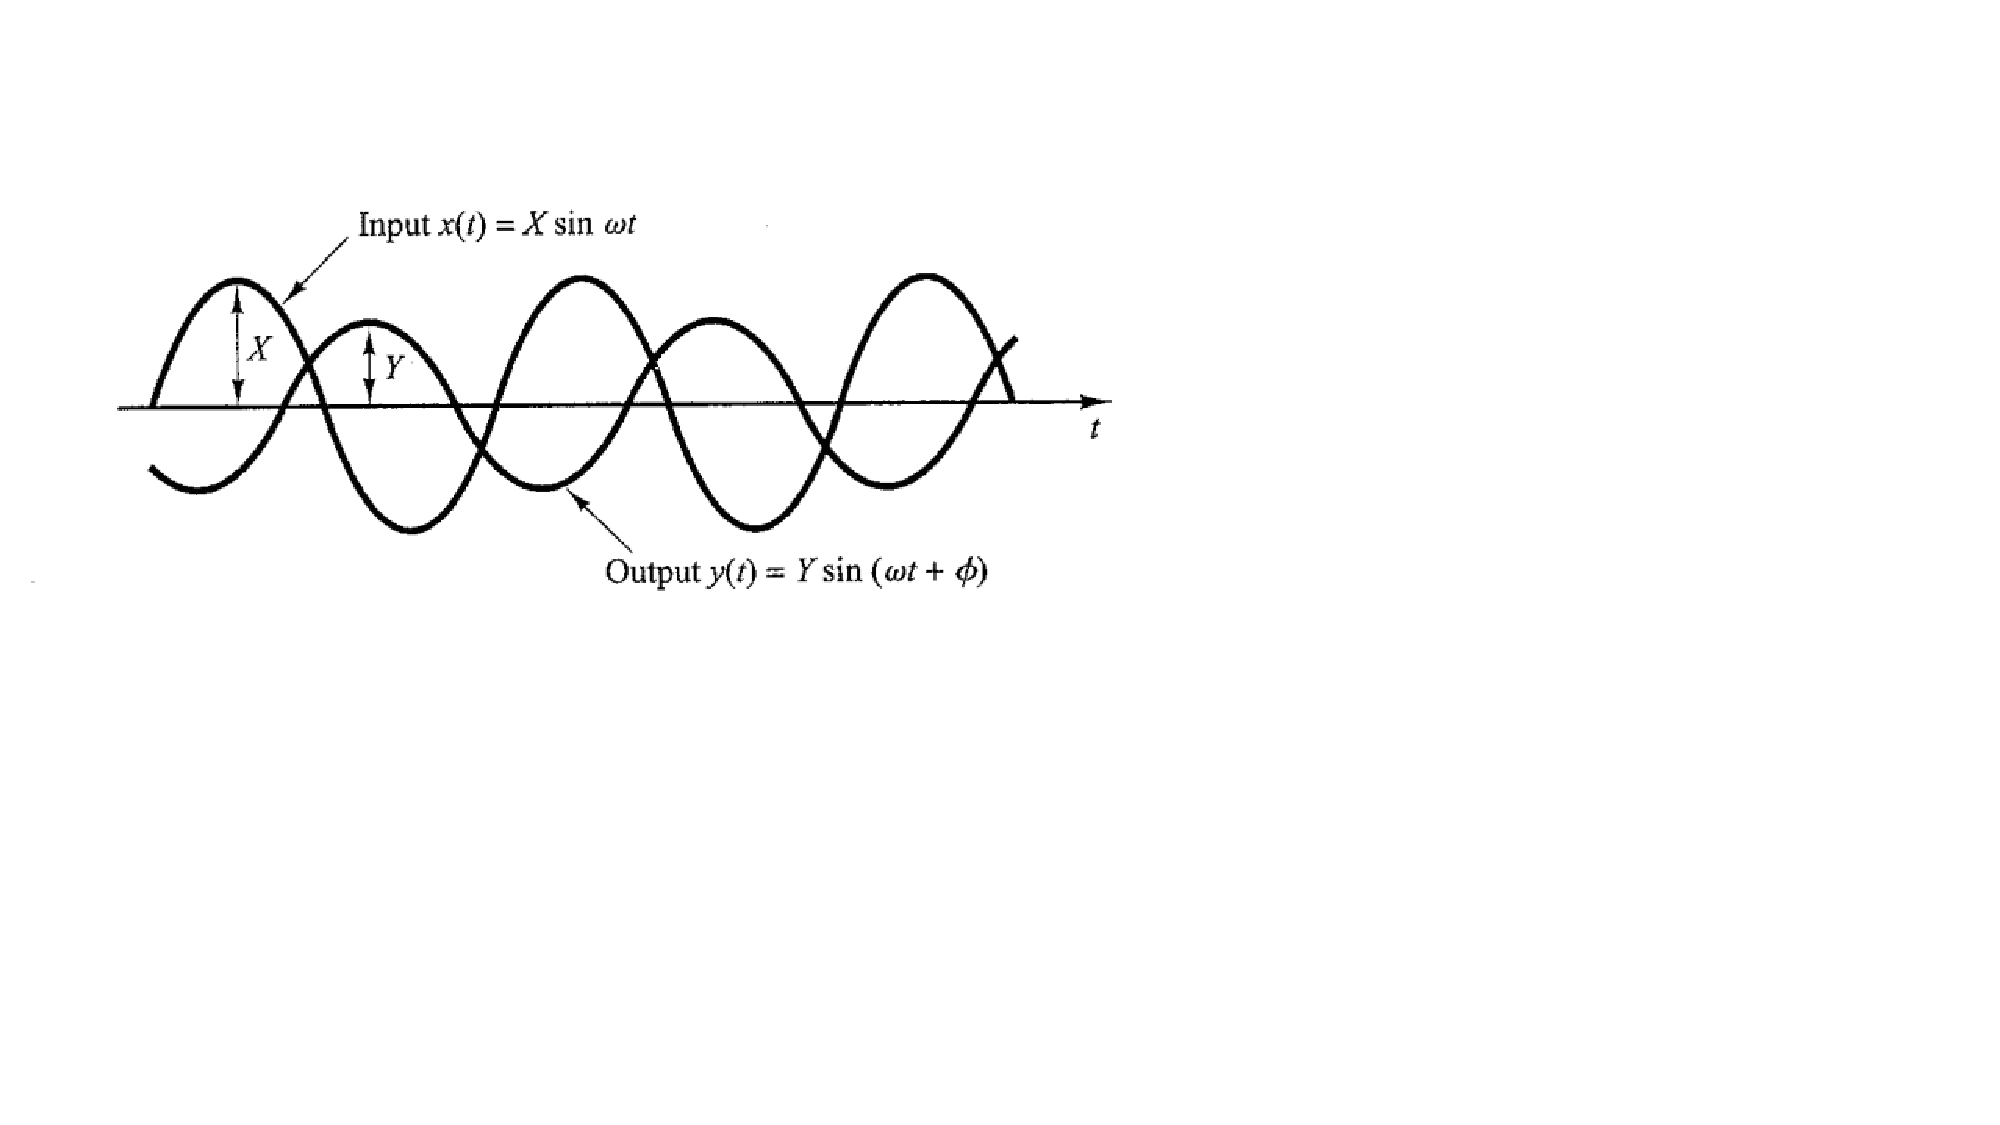
\includegraphics[scale=0.5]{IOSinus}


\begin{itemize}
\item $|H(j\omega)| = \frac{Y}{X}$ and $\phi = \angle H(j\omega)$ can directly be found in the bode plot at frequency $\omega$
\end{itemize}

\end{frame}

\section{What Is A Bode Plot}

\begin{frame}
\frametitle{The bode plot}
\begin{definition}
	\begin{itemize}
		\item A bode plot is a graphical representation of the sinusoidal transfer function $H(j\omega)$
		\item It consists of two separate plots, a magnitude and a phase plot
		\item In this way, we can see the relation of a sinusoidal input with a given frequency $\omega$ to a linear system and its output
		\item After all, the relation between the amplitudes is given by $|H(j\omega)|$ and the phase shift by $\angle H(j\omega)$
		
	\end{itemize}
\end{definition}



\end{frame}


\begin{frame}
\frametitle{Example bode plot}

	\begin{columns}
		\begin{column}{0.5\textwidth}
			$H(s) = \frac{14s^2 + 7s + 3}{s^4 + 10s^3 + 10s^2 + 10s + 10}$\\
			\vspace{10mm}
			\begin{itemize}
				\item Say we use an input $x(t) = 2\sin(100t)$ in this system.
				\item The steady state response would be 
				\vspace{5mm} $$y(t) = |H(j100)|\cdot 2\sin\Big(100t + \angle H(j100)\Big)$$
			\end{itemize}
		\end{column}
		
		\begin{column}{0.5\textwidth}
			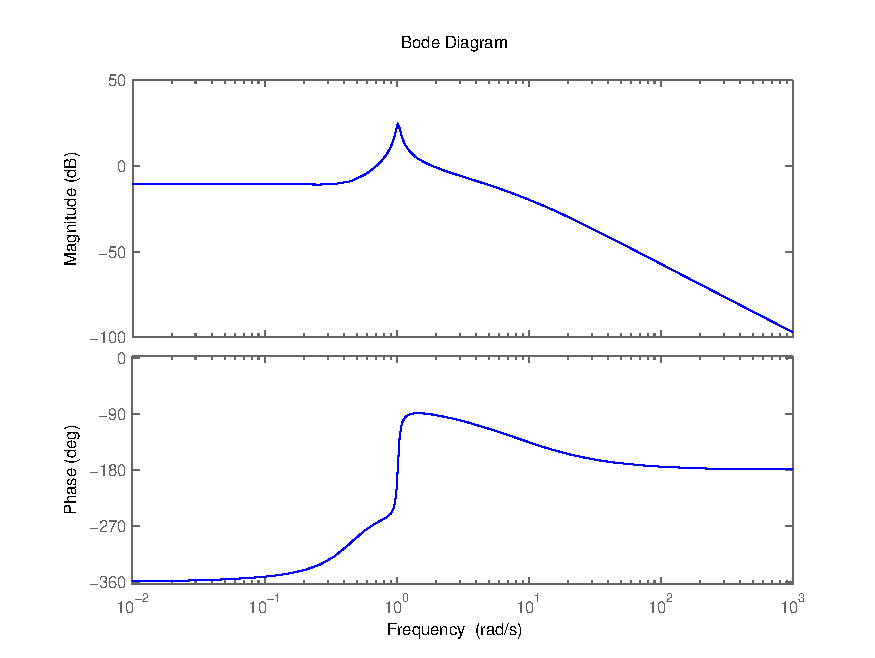
\includegraphics[scale=0.4]{ExampleBode1}
		\end{column}
		
	\end{columns}



\end{frame}



\begin{frame}
\frametitle{The magnitude plot}

Convention: 
\begin{itemize}
\item for the ordinate (y-axis) we use $20\log_{10}|H(j\omega)|$ with the unit $dB$
\item for the abscissa (x-axis) we use a logarithmic plot of $\omega$

\end{itemize}
This is thus a bi-log plot

The reason for using the logarithm of the modulus of $H(j\omega)$ will become clear later

\end{frame}




\begin{frame}
\frametitle{The phase plot}
Convention:
\begin{itemize}
\item for the ordinate (y-axis) we use $\angle H(j\omega)$ in degrees
\item for the abscissa (x-axis) we use a logarithmic plot of $\omega$

\end{itemize}
This is thus a semi-log plot


\end{frame}



\begin{frame}
\frametitle{Discrete time systems}

\begin{itemize}
\item The transfer function is a function of $z$, i.e. $H(z)$.
\item In contrast to continuous time systems, we do not use $H(j\omega)$. Instead, $H(e^{j\omega T_s})$ is now the sinusoidal transfer function.
\item $T_s$ is the sample time, i.e. the amount of time in between each sample.
\end{itemize}


\end{frame}

\section{How To Construct A Bode Plot (by hand)}

\begin{frame}
\frametitle{A new representation of the transfer function}
From before:
\begin{align*}
H(s) &= \frac{\beta_0 s^r + \beta_1 s^{r-1} + \ldots + \beta_r}{s^n + \alpha_1 s^{n-1} + \ldots + \alpha_n}\\
\text{Factorization in zeros and poles}\\
\Rightarrow \quad
H(s) &= \frac{\beta_0 (s-n_1) (s-n_2) \ldots (s-n_r)}{(s-p_1) (s-p_2) \ldots (s-p_n)}
\end{align*}
This is the usual representation. Now however, we will look for factors $(1+\displaystyle{\frac{s}{s_i}})$, with $s_i$ a so-called breakpoint.


\end{frame}


\begin{frame}
\frametitle{A new representation of the transfer function}
We can do this by bringing all the zeros and poles not equal to zero outside the brackets, as follows:
$$H(s) = \beta_0 \frac{\prod(-n_i)}{\prod(-p_j)} \frac{(1+\frac{s}{-n_1}) (1+\frac{s}{-n_2}) \ldots (1+\frac{s}{-n_i})}{s^l (1+\frac{s}{-p_1}) (1+\frac{s}{-p_2}) \ldots (1 + \frac{s}{-p_j})}$$
 Replacing the constants by $K$, and setting $$r_k = -n_k$$ $$ s_k = -p_k$$ 



\end{frame}



\begin{frame}
\frametitle{A new representation of the transfer function}

We ultimately get: $$H(s) = K \frac{(1+\frac{s}{r_1}) (1+\frac{s}{r_2}) \ldots (1+\frac{s}{r_i})}{s^l (1+\frac{s}{s_1}) (1+\frac{s}{s_2}) \ldots (1 + \frac{s}{s_j})}$$
Now we are able to construct the bode plot of each different factor of $H(s)$. Afterwards we can just add up these plots using the calculation rules of complex numbers.

  
\end{frame}



\begin{frame}
\frametitle{Intermezzo complex numbers}
\begin{itemize}
\item The magnitude of the product of complex numbers is equal to the product of the magnitudes of these numbers
\item The phase of the product of complex numbers is equal to the sum of the phases of these numbers
\item The logarithm of a product of numbers is equal to the sum of the logarithms of these numbers

\end{itemize}
This comes down to 
$$ 20\log_{10}|H(j\omega)| = \sum 20\log_{10}|\text{factors}| $$ 
$$ \angle H(j\omega) = \sum(\angle \text{factors})$$

Next we will quickly go over the simple bode plots of the different factors of $H(s)$

\end{frame}



\begin{frame}
\frametitle{The constant K}
\begin{itemize}
\item $20\log_{10}|K| =$ constant
\item $\angle K = 0^{\circ} \text{ or} \pm 180^{\circ}$  (resp. $K > 0$ and $K < 0$)
\end{itemize}
Example: $K = 10$

\begin{center}
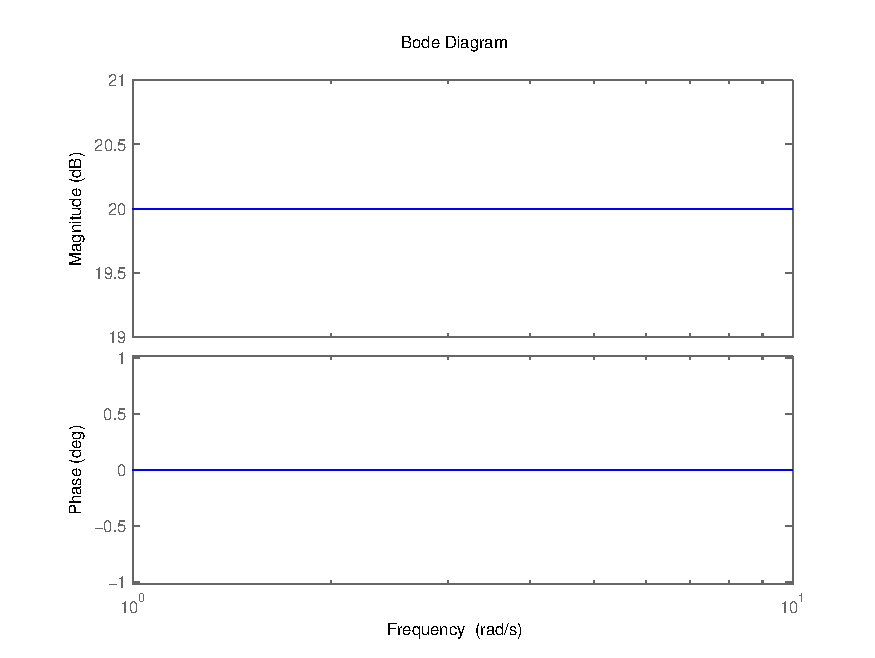
\includegraphics[scale=0.45]{BodeConstant}
\end{center}

\end{frame}



\begin{frame}
\frametitle{$(1+\frac{j\omega}{r_i})$ in the numerator}
(Assume $r_i > 0$)
\begin{itemize}
\item What if $\omega \rightarrow 0$ ? \quad $(1+\frac{j\omega}{r_i}) \rightarrow 1$
\begin{itemize}
\item $20\log_{10}|1| = 0$
\item $\angle 1 = 0^{\circ}$
\end{itemize}

\item What if $\omega \rightarrow \infty$ ?  \quad  $(1+\frac{j\omega}{r_i}) \rightarrow j\infty$
\begin{itemize}
\item $20\log_{10}|j\infty| = \infty$
\item $\angle j\infty = 90^{\circ}$
\end{itemize}

\item The two terms balance each other out for $\omega = r_i$ (remember, this is called a breakpoint).
\begin{itemize}
\item $20\log_{10}|1+j| = 20\log_{10}(\sqrt 2) \approx 3 \text{dB}$
\item $\angle(1+j) = 45^{\circ}$
\end{itemize}
\end{itemize}
A breakpoint is therefore also called a 3dB point
\end{frame}



\begin{frame}
\frametitle{$(1+\frac{j\omega}{r_i})$ in the numerator}
Example: $r_i = 100$

\begin{center}
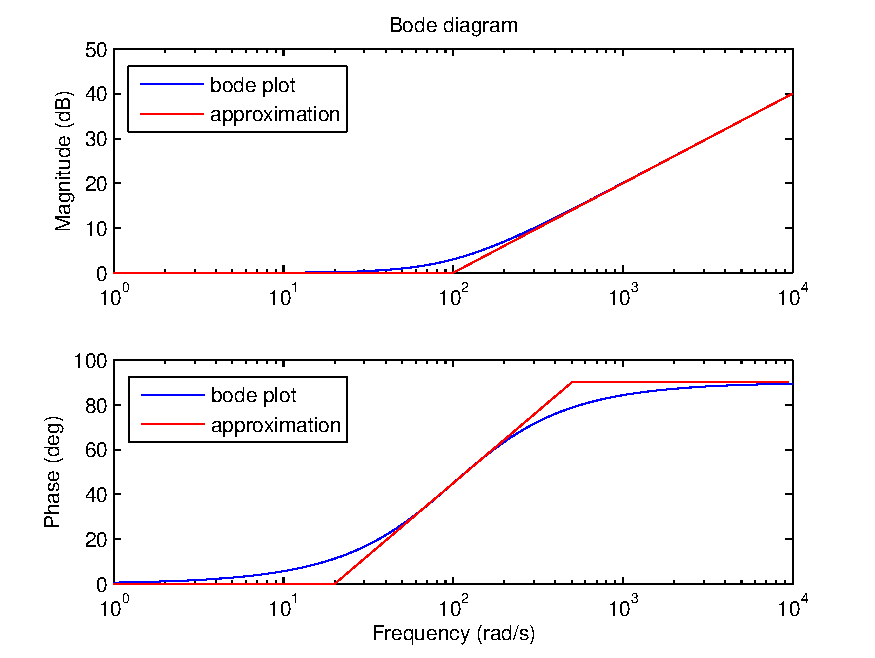
\includegraphics[scale=0.5]{BodeNumerator}
\end{center}

\end{frame}



\begin{frame}
\frametitle{$(1+\frac{j\omega}{s_i})$ in the denominator}
This factor is equivalent to the previous one. The only difference is the sign change in both plots:

\begin{itemize}
\item What if $\omega \rightarrow 0$ ? \quad $\frac{1}{1+\frac{j\omega}{s_i}} \rightarrow 1$
\begin{itemize}
\item $20\log_{10}|1| = 0$
\item $\angle 1 = 0^{\circ}$
\end{itemize}

\item What if $\omega \rightarrow \infty$ ?  \quad  $\frac{1}{1+\frac{j\omega}{s_i}} \rightarrow \frac{1}{j\infty} \rightarrow -j0$
\begin{itemize}
\item $20\log_{10}|-j0| = -\infty$
\item $\angle -j0 = -90^{\circ}$
\end{itemize}

\item The two terms balance each other out for $\omega = s_i$
\begin{itemize}
\item $20\log_{10}\frac{1}{|1+j|} = 20\log_{10}(\frac{1}{\sqrt 2}) \approx -3 \text{dB}$
\item $\angle\frac{1}{(1+j)} = -45^{\circ}$
\end{itemize}
\end{itemize}
%\begin{itemize}
%\item $\log |\frac{1}{z}| = -\log|z|$
%\item $\angle \frac{1}{z} = -\angle z$
%\end{itemize}


\end{frame}


\begin{frame}
\frametitle{$(1+\frac{j\omega}{s_i})$ in the denominator}
Example $s_i = 100$

\begin{center}
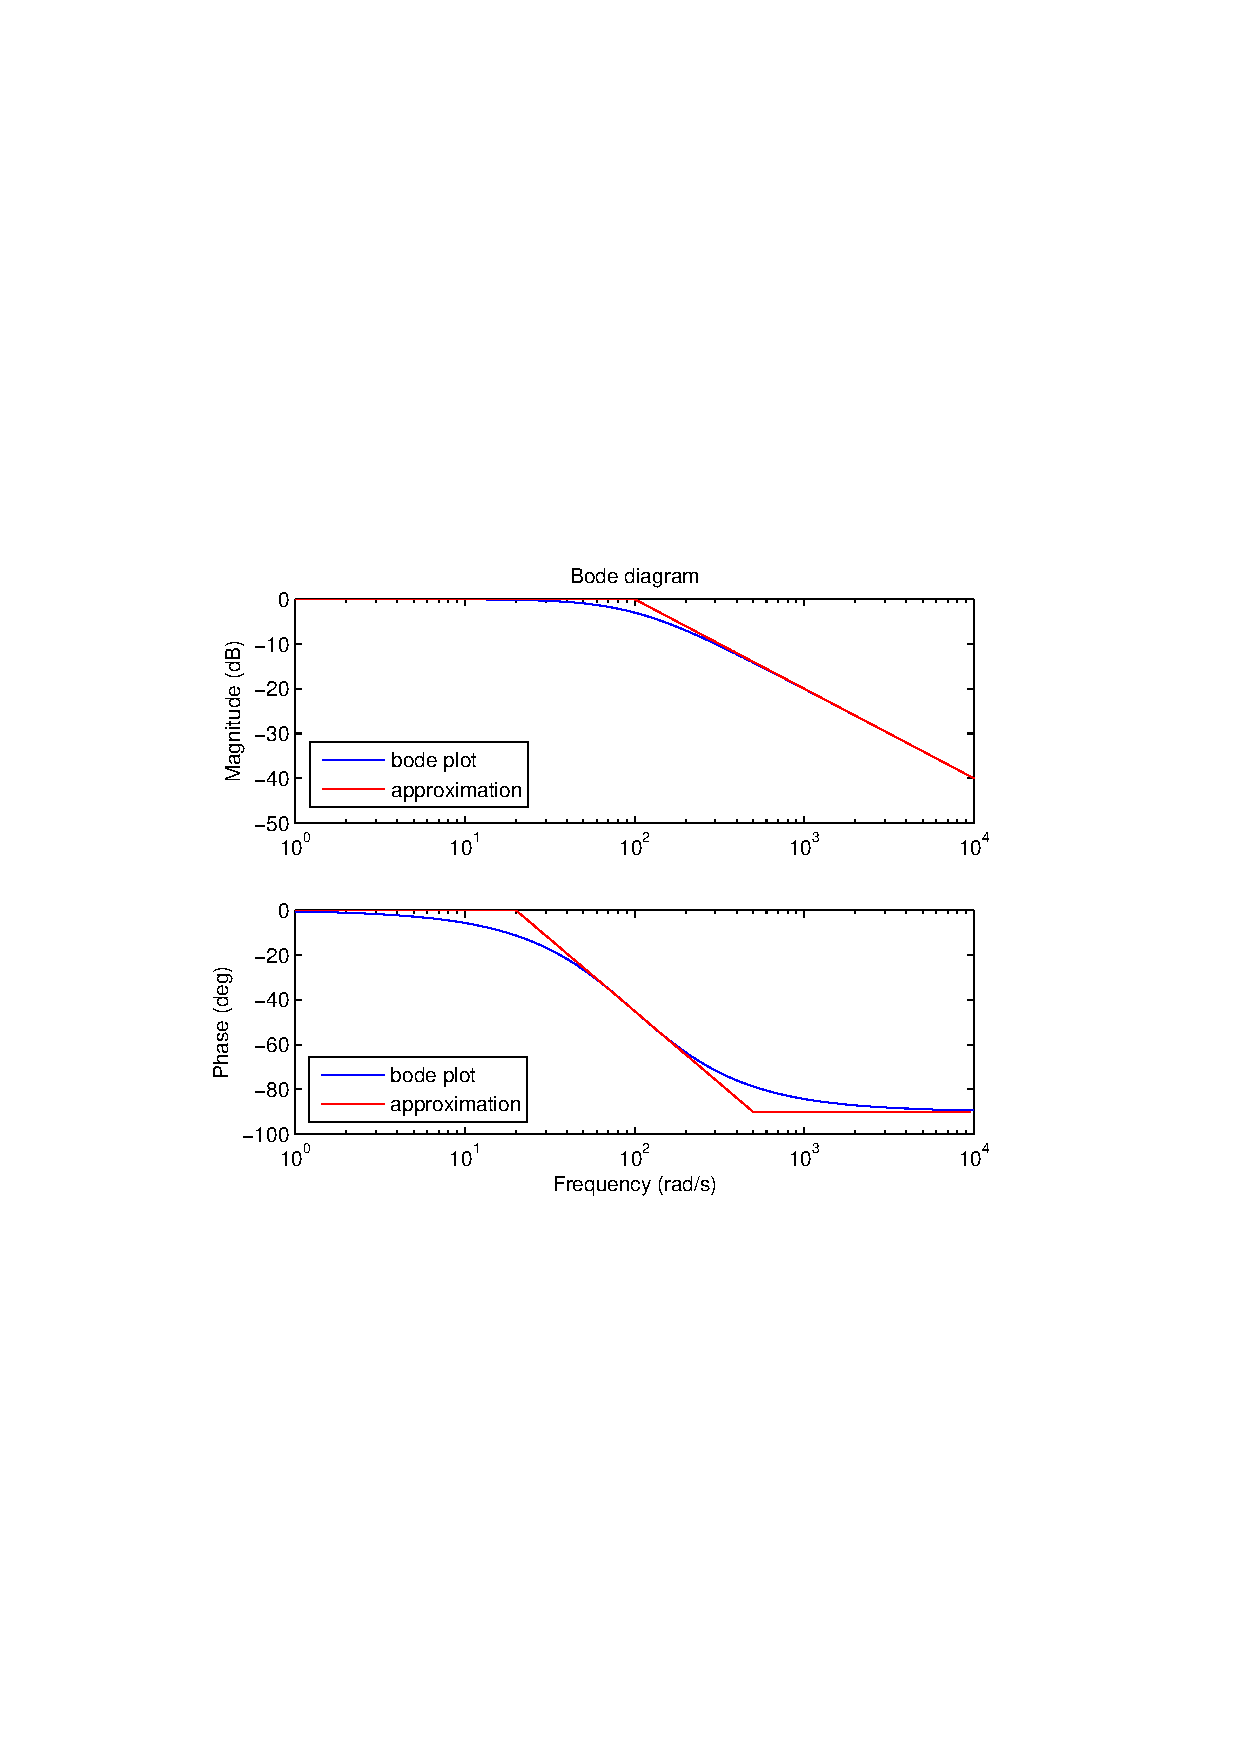
\includegraphics[scale=0.5]{BodeDenominator}
\end{center}

\end{frame}


\begin{frame}
\frametitle{$j\omega$ in the numerator}

\begin{itemize}
\item This is simply a (ascending) straight line in the magnitude plot, with a slope of 20 dB/decade
\item Constant phase of $90^{\circ}$
\end{itemize}

\begin{itemize}
\item What if $\omega \rightarrow 0$ ? \quad $j\omega \rightarrow j0$
\begin{itemize}
\item $20\log_{10}|j0| = -\infty$
\item $\angle j0 = 90^{\circ}$
\end{itemize}

\item What if $\omega \rightarrow \infty$ ?  \quad  $j\omega \rightarrow j\infty$
\begin{itemize}
\item $20\log_{10}|j\infty| = \infty$
\item $\angle j\infty = 90^{\circ}$
\end{itemize}
\end{itemize}

\end{frame}

\begin{frame}
\frametitle{$j\omega$ in the numerator}

\begin{center}
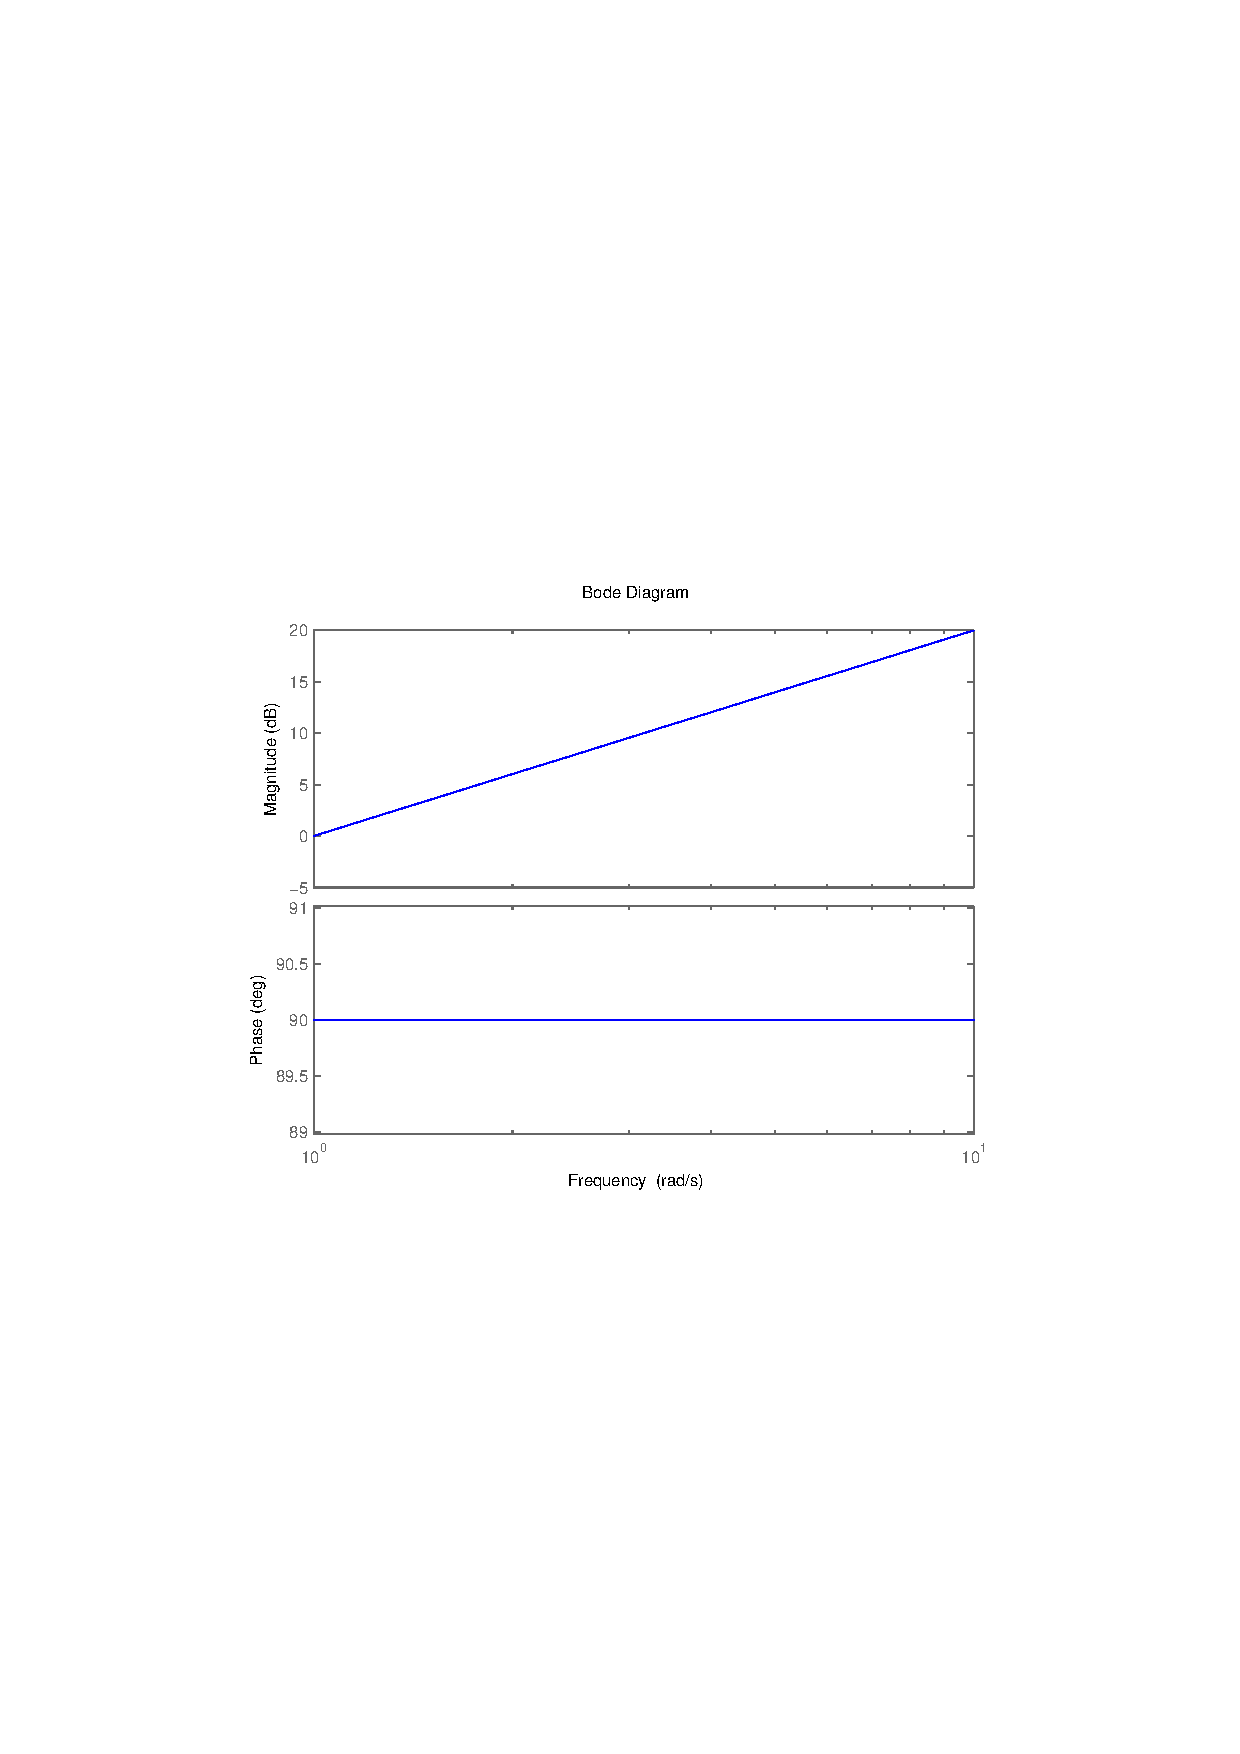
\includegraphics[scale=0.5]{BodeZeroNum}
\end{center}

\end{frame}

\begin{frame}
\frametitle{$j\omega$ in the denominator}

\begin{itemize}
\item This is simply a (descending) straight line in the magnitude plot, with a slope of -20 dB/decade
\item Constant phase of $-90^{\circ}$
\end{itemize}

\begin{itemize}
\item What if $\omega \rightarrow 0$ ? \quad $\frac{1}{j\omega} \rightarrow \frac{1}{j0} \rightarrow -j\infty$
\begin{itemize}
\item $20\log_{10}|-j\infty| = \infty$
\item $\angle -j\infty = -90^{\circ}$
\end{itemize}

\item What if $\omega \rightarrow \infty$ ?  \quad  $\frac{1}{j\omega} \rightarrow \frac{1}{j\infty} \rightarrow -j0$
\begin{itemize}
\item $20\log_{10}|-j0| = -\infty$
\item $\angle -j0 = -90^{\circ}$
\end{itemize}
\end{itemize}

\end{frame}

\begin{frame}
\frametitle{$j\omega$ in the denominator}

\begin{center}
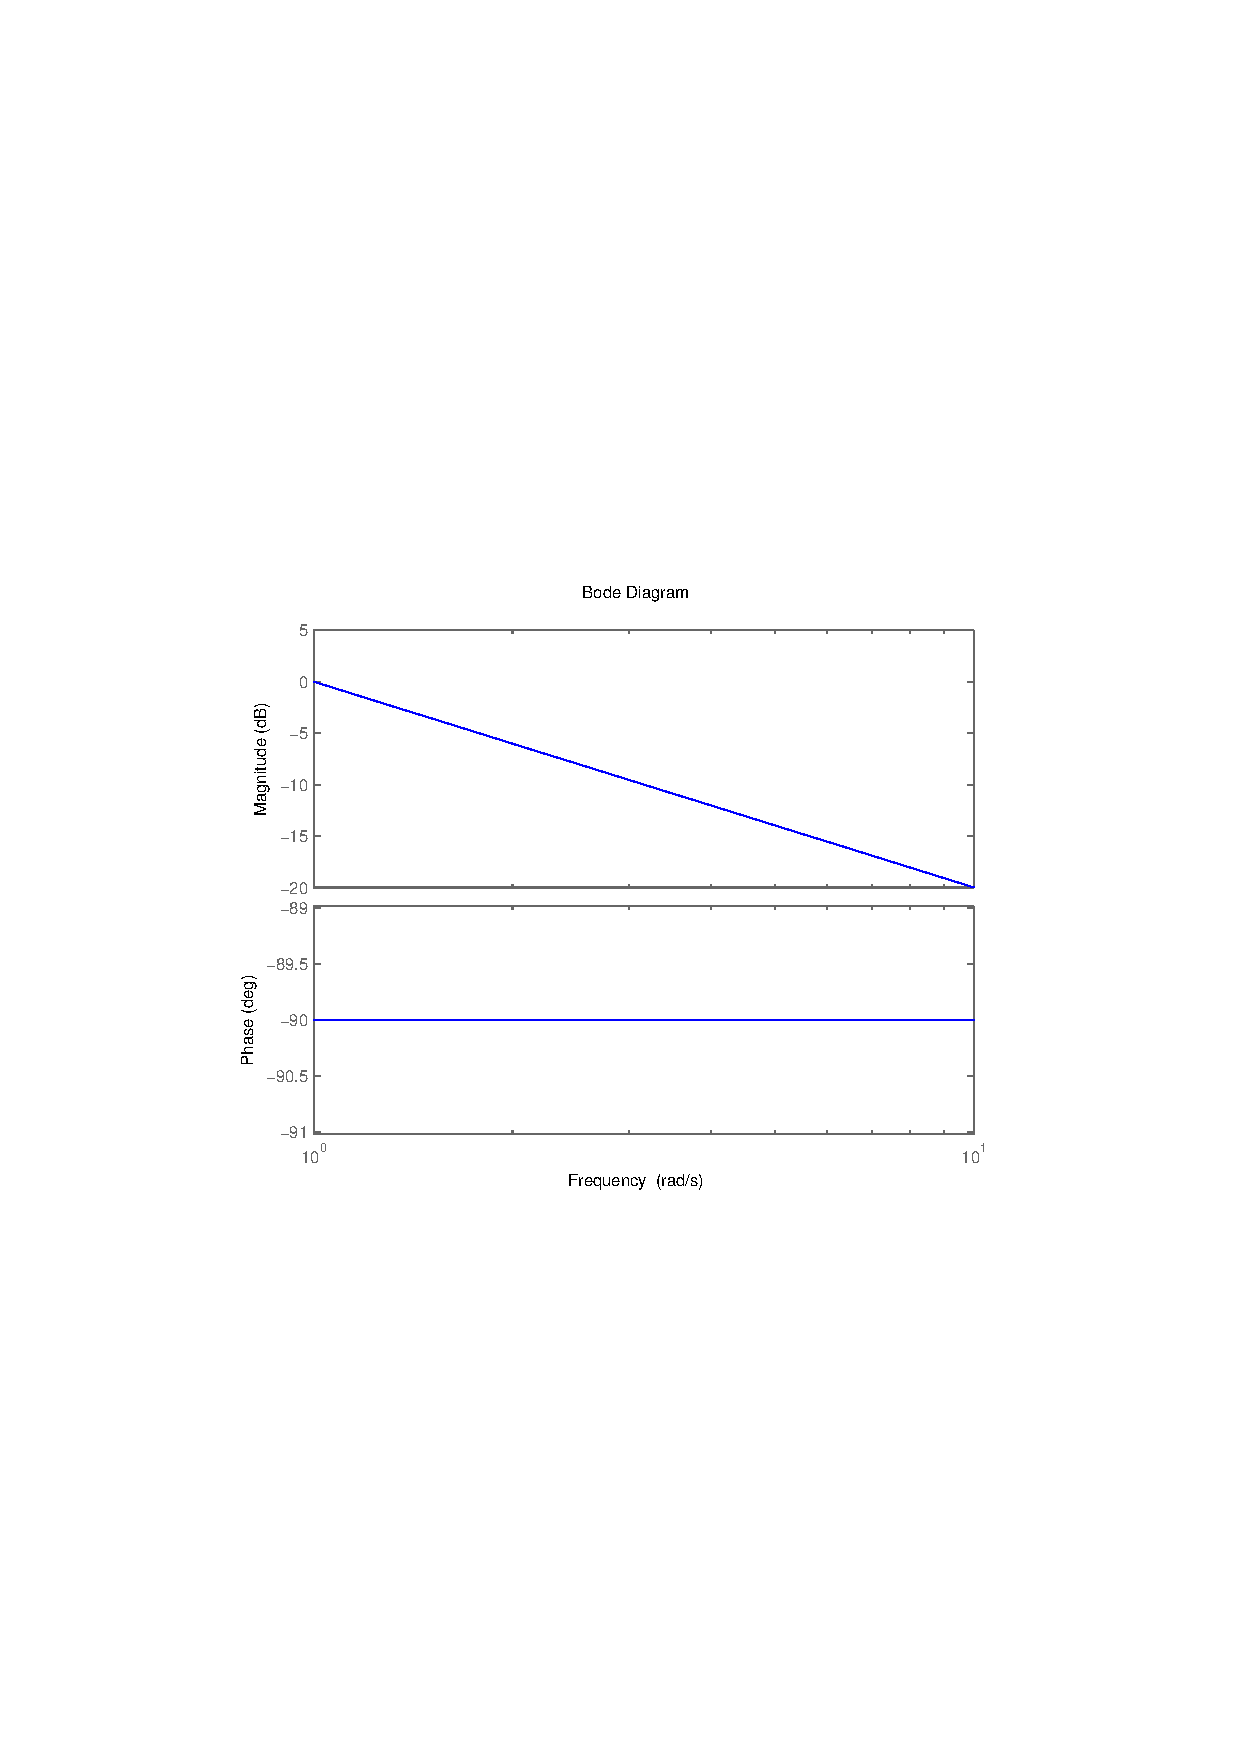
\includegraphics[scale=0.5]{BodeZeroDen}
\end{center}

\end{frame}



\begin{frame}
\frametitle{What if the multiplicity is higher than 1?}

Take for example multiplicity 2, a second order factor.\\
A second order factor has twice the effect of a first order factor.\\
Consider for example the effect of a double zero:
\begin{itemize}
\item Slope of 40dB/decade instead of 20dB/decade after the breakpoint
\item Phase shift of $180^{\circ}$ instead of $90^{\circ}$

\end{itemize}
\end{frame}

\begin{frame}
\frametitle{Second order factor}
$(1+\frac{j\omega}{100})^2$

\begin{center}
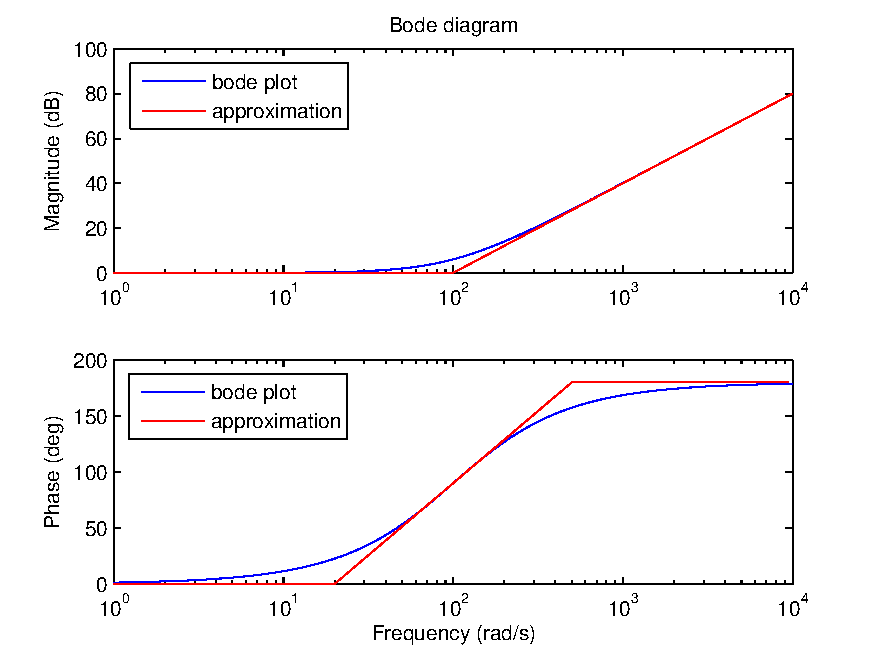
\includegraphics[scale=0.5]{BodeSecondOrder}
\end{center}


\end{frame}


\begin{frame}
\frametitle{Exception}
\begin{alertblock}{Exception}
	Up until now we always considered $r_i \text{ and } s_i > 0$, but what if we have a factor $(1-\frac{j\omega}{r_i})$ for example?
	\begin{itemize}
		\item The magnitude plot remains unchanged, as $|1+\frac{j\omega}{r_i}| = |1 - \frac{j\omega}{r_i} |$
		\item The phase plot is reversed, as $\angle(1+\frac{j\omega}{r_i}) = -\angle(1 - \frac{j\omega}{r_i})$
		\item If we have such a factor in the denominator, the system will be unstable!
	\end{itemize}
	
\end{alertblock}

\end{frame}


\begin{frame}
\frametitle{Exception}
Example $(1 - \frac{j\omega}{100})$ in the numerator

\begin{center}
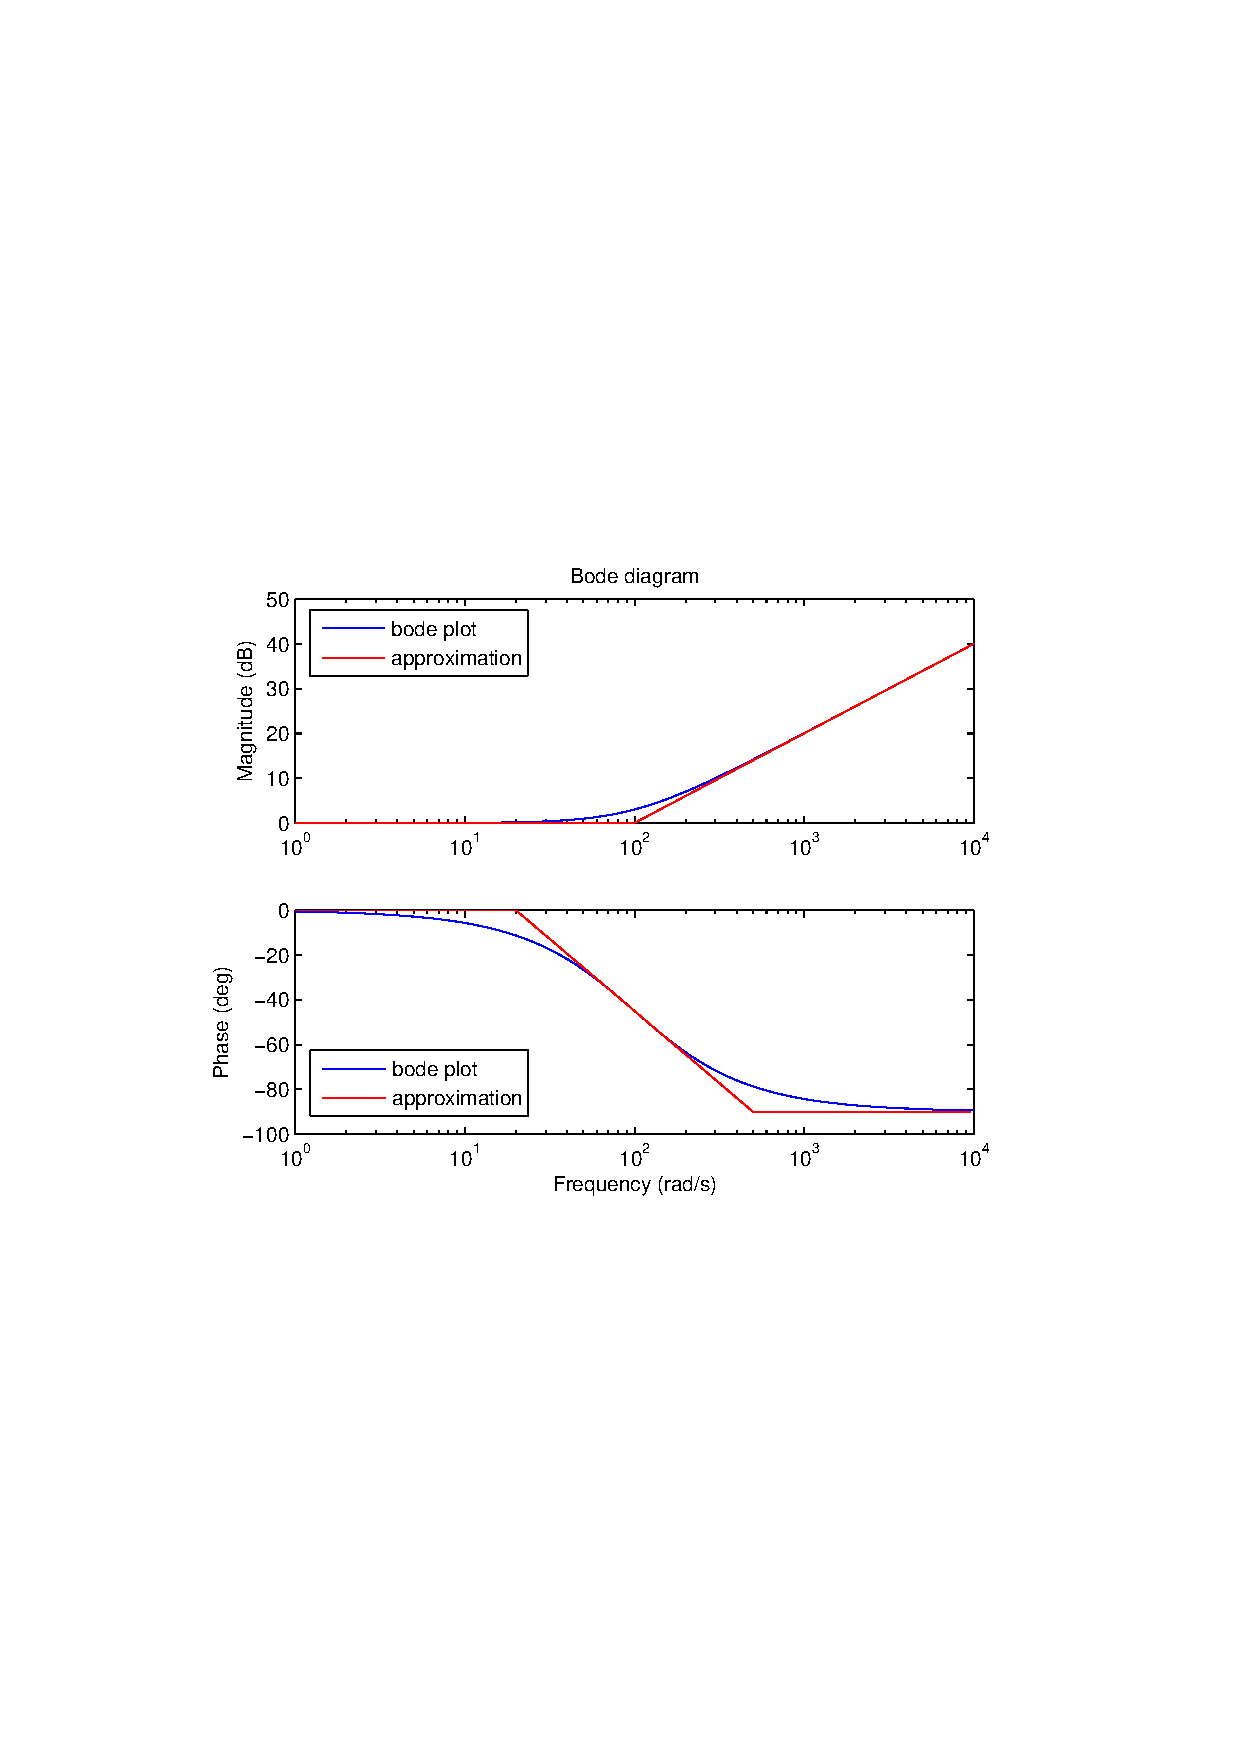
\includegraphics[scale=0.5]{BodeException}
\end{center}

\end{frame}


\begin{frame}
\frametitle{Quadratic factors and resonance}
\begin{itemize}
Also possible is a quadratic factor $[1 + 2\zeta(j\frac{\omega}{\omega_n}) +  (j\frac{\omega}{\omega_n})^2]^{\pm1}$
\item $\zeta$ is called the damping factor, $\omega_n$ is the natural frequency
\item If $\zeta > 1$, this quadratic factor can be expressed as two first order factors with real zeros/poles
\item But if $0 < \zeta < 1 $, this quadratic factor is the product of two complex-conjugate factors
\item For low $\zeta$, the asymptotic approximations are not accurate. Instead, a peak occurs in the magnitude plot around $\omega_n$
\item This peak is a phenomenon known as resonance. 
\end{itemize}

\end{frame}

\begin{frame}
\frametitle{Quadratic factors and resonance}

\begin{columns}
\begin{column}{0.19\textwidth}
\end{column}
\begin{column}{0.81\textwidth}
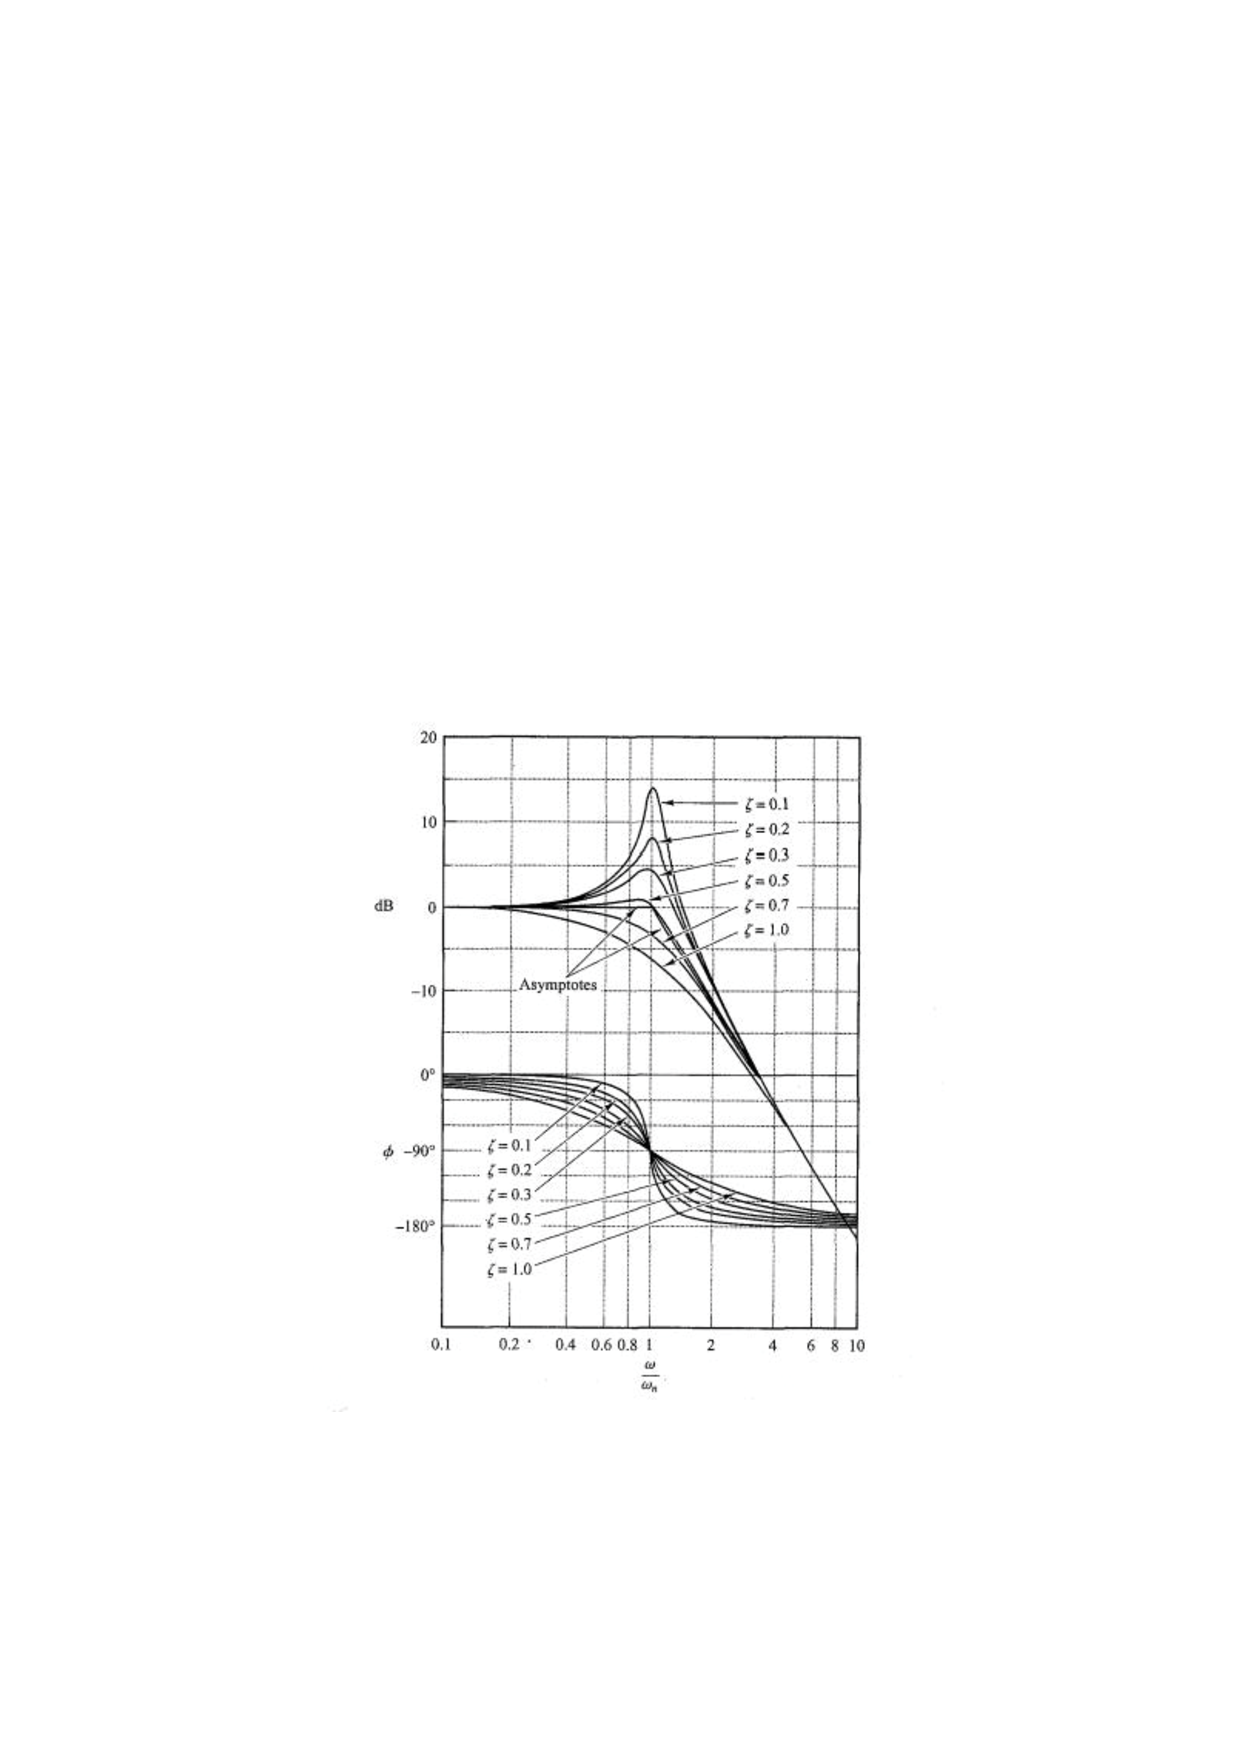
\includegraphics[scale = 0.35]{Resonance}
\end{column}
\end{columns}


\end{frame}


\begin{frame}
\frametitle{Example}

	Suppose we want to construct (by hand) the bode plot of $$H(s) = \frac{s^2 + 1100s + 100000}{10s^3 + 200s^2 + 1000s}$$
	
	The first step is to find the representation with breakpoints.
	\begin{align*}
	H(s) &=  \frac{s^2 + 1100s + 100000}{10s^3 + 200s^2 + 1000s}\\
	&= \frac{(s+100)(s+1000)}{10s(s+10)^2}\\
	&= \frac{100000(1+\frac{s}{100})(1+\frac{s}{1000})}{1000s(1+\frac{s}{10})^2}
	&= \frac{100(1+\frac{s}{100})(1+\frac{s}{1000})}{s(1+\frac{s}{10})^2}
	\end{align*}



\end{frame}

\begin{frame}
\frametitle{Example Magnitude plot}
\begin{center}
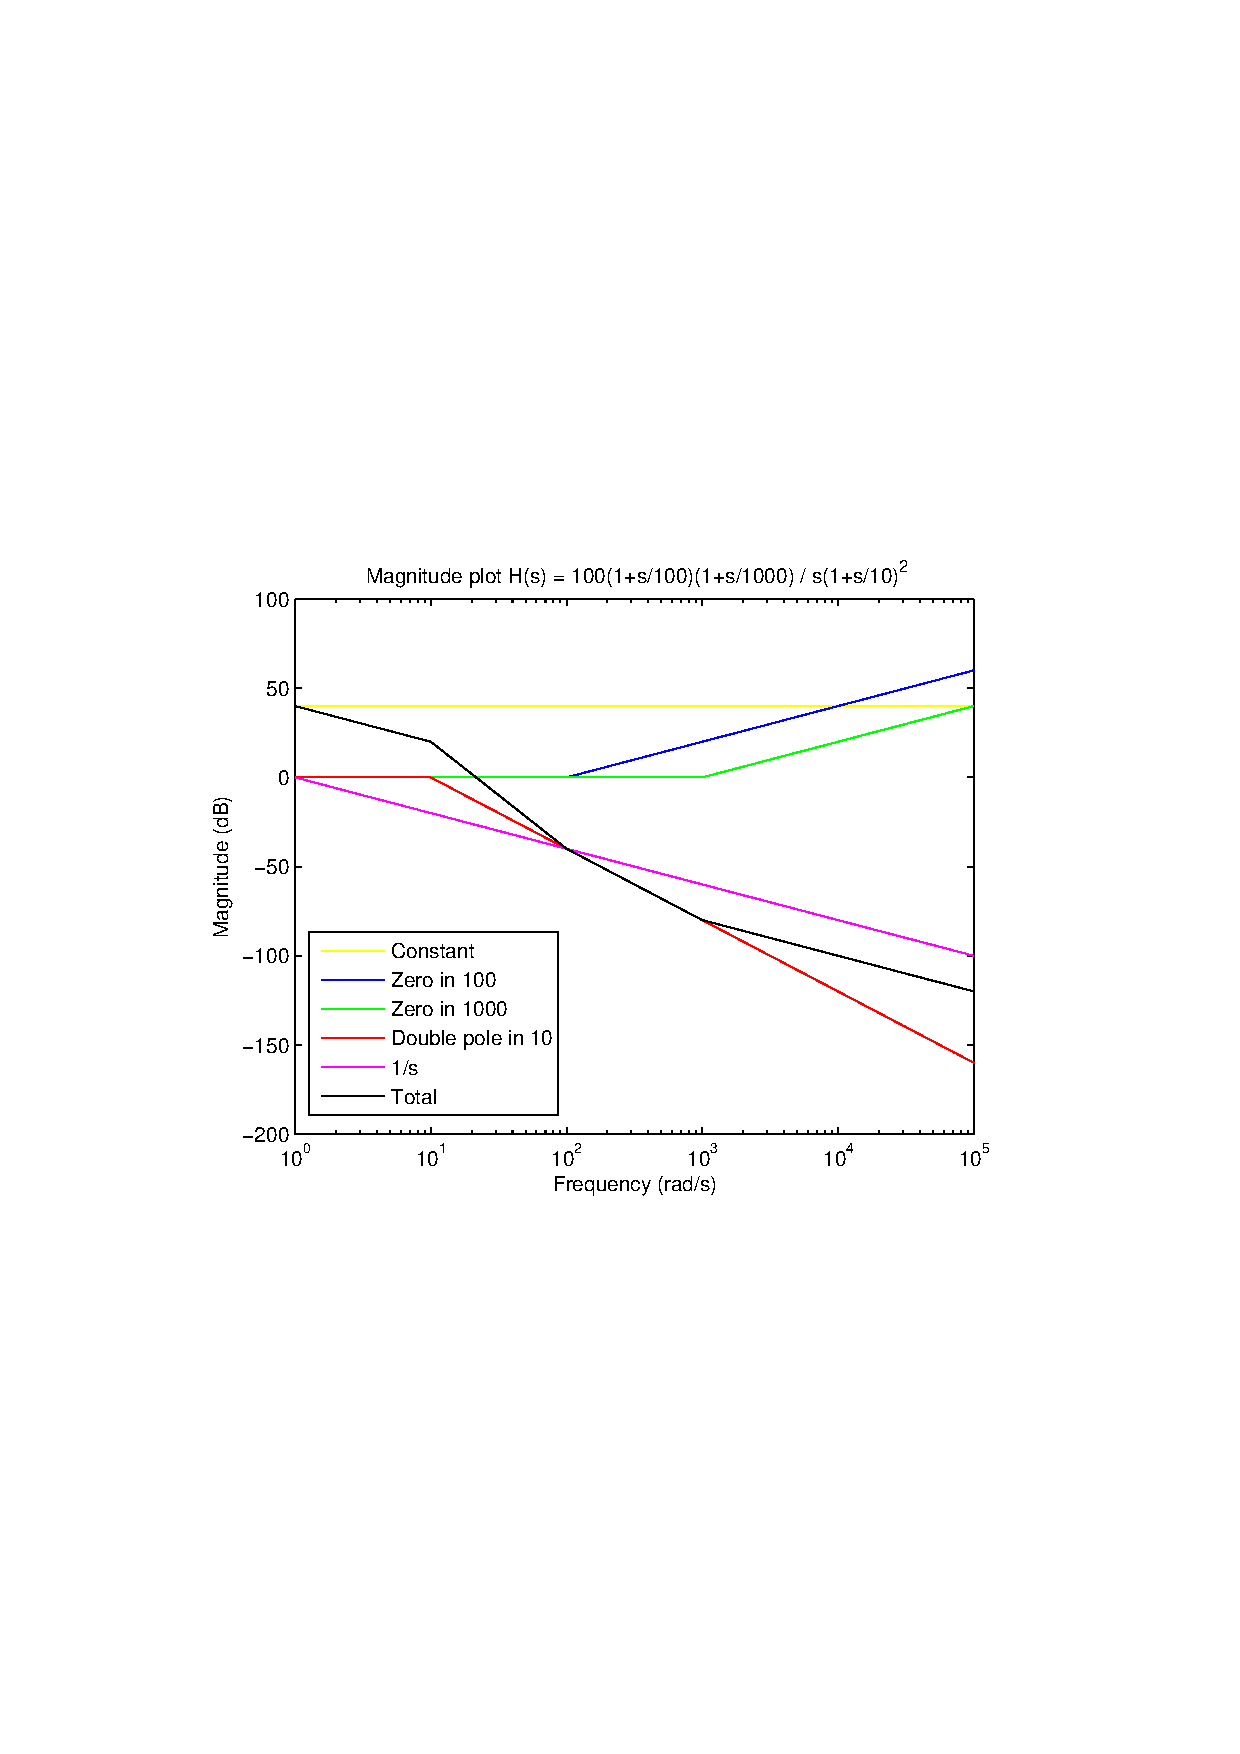
\includegraphics[width=0.7\linewidth]{MagnitudeParts}
\end{center}
\end{frame}

\begin{frame}
\frametitle{Example Magnitude plot}

\begin{center}
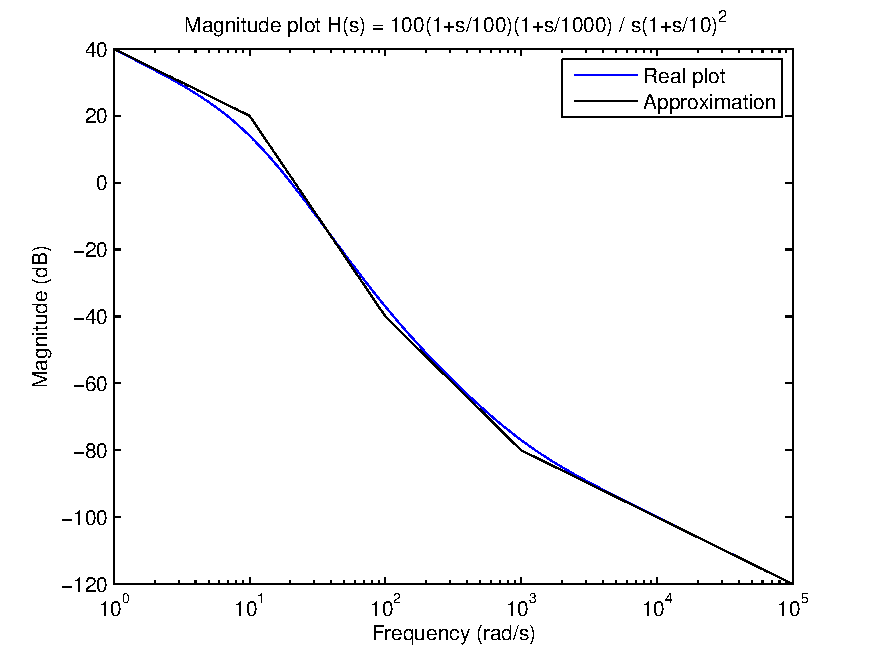
\includegraphics[scale=0.5]{MagnitudeApprox}
\end{center}


\end{frame}

\begin{frame}
\frametitle{Example Phase plot}

\begin{center}
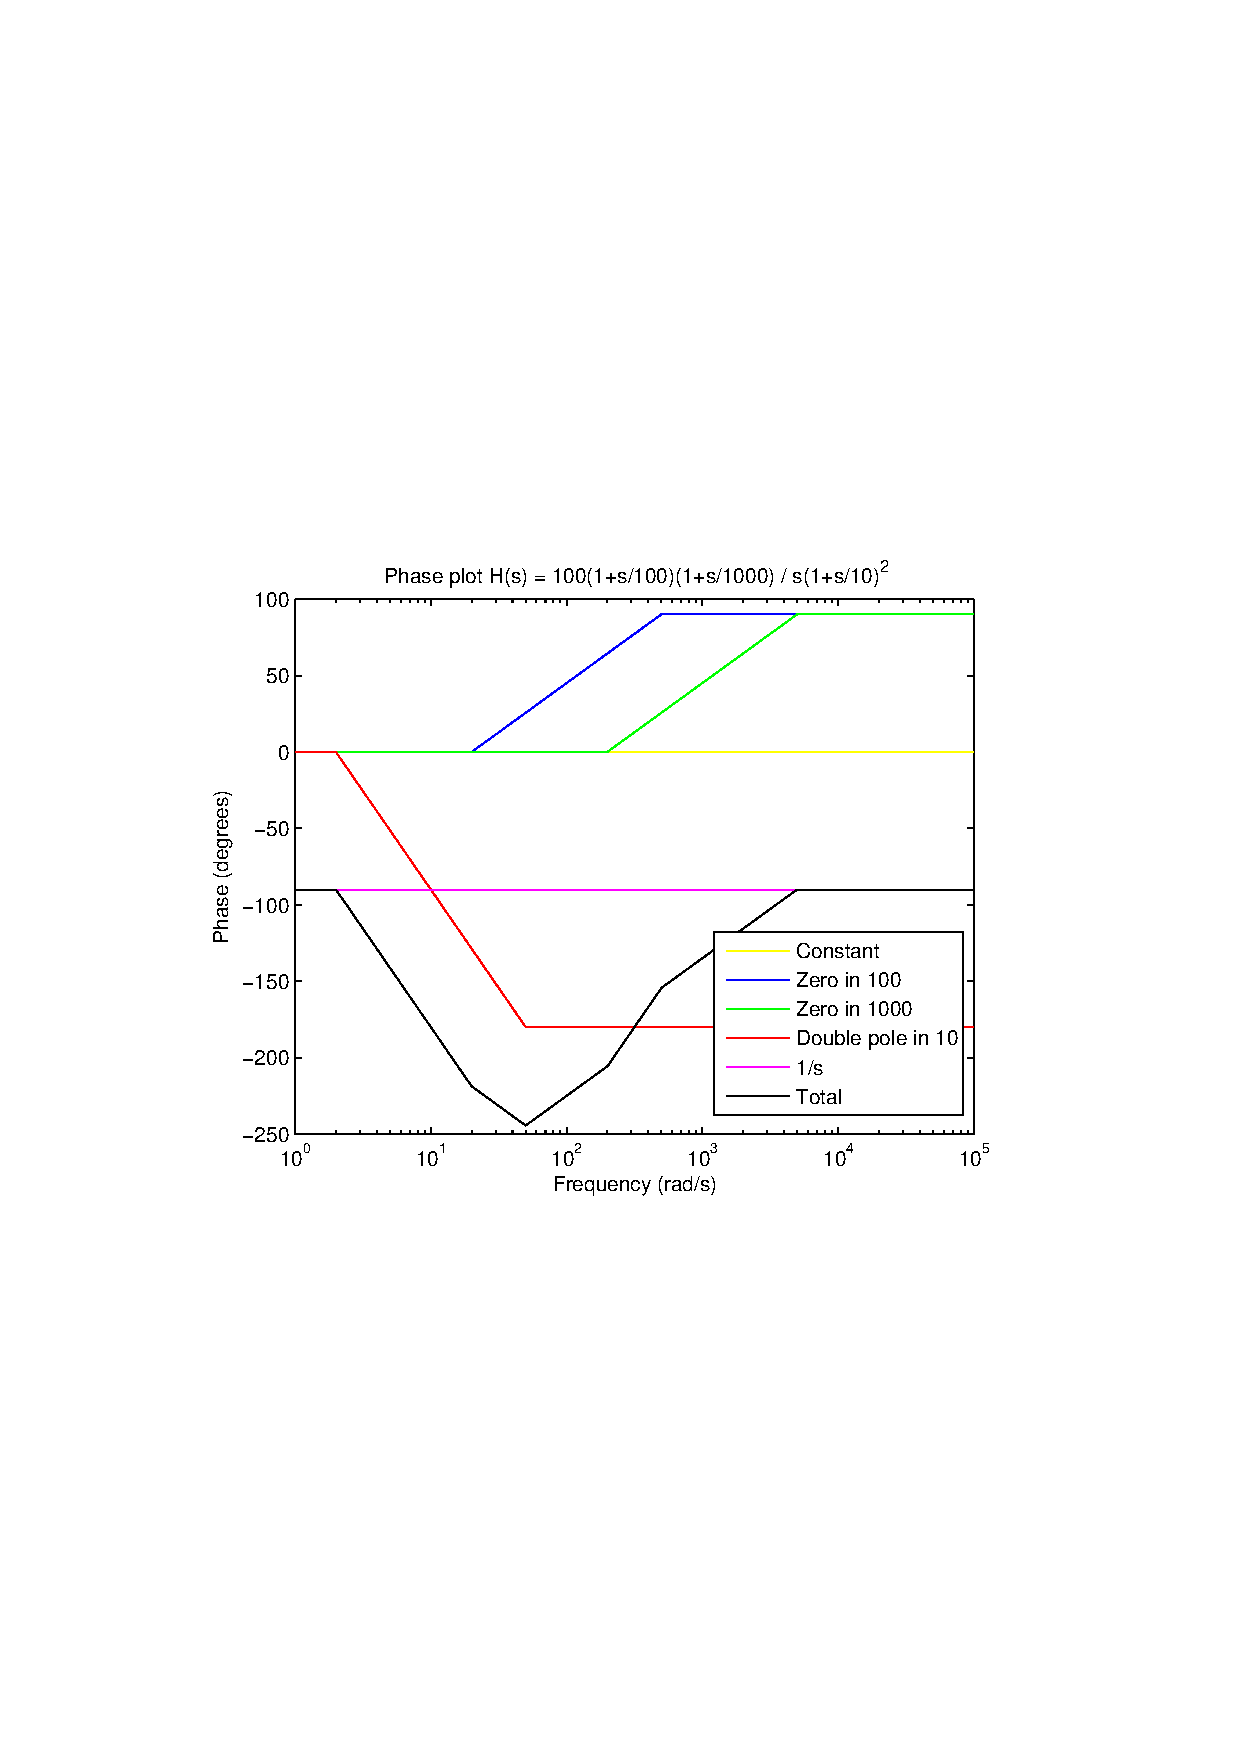
\includegraphics[scale=0.5]{PhaseParts}
\end{center}


\end{frame}

\begin{frame}
\frametitle{Example Phase plot}

\begin{center}
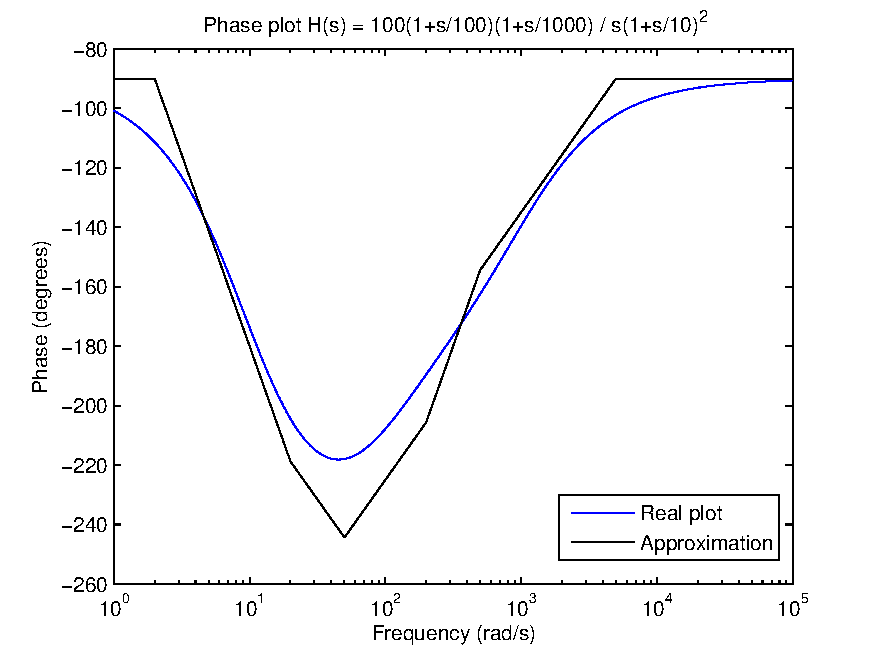
\includegraphics[scale=0.5]{PhaseApprox}
\end{center}


\end{frame}

\section{Constructing The Bode Plot In Matlab}

\begin{frame}
\frametitle{Basic commands in Matlab}

In Matlab it is very easy to draw the bode plot:
\begin{itemize}
\item First, define the system using one of the following commands:
	\begin{itemize}
	\item \textcolor{blue}{tf(num,den)} (\textcolor{blue}{num} and \textcolor{blue}{den} are respectively the numerator and denominator of the transfer function)
	\item \textcolor{blue}{zpk(z,p,K)} (using the zeros (\textcolor{blue}{z}), the poles (\textcolor{blue}{p}) and the gain (\textcolor{blue}{K}) of the transfer function)
	\item \textcolor{blue}{ss(A,B,C,D)} (using the matrices of the state-space model)

	\end{itemize}
\item In case of a discrete time system, \textcolor{blue}{Ts} (the sample time) is also needed as a last parameter in these commands
\item Next, use the command \textcolor{blue}{bode(sys)}

\end{itemize}

\end{frame}

\begin{frame}
\frametitle{Matlab example}
\lstinputlisting{CreateBodeMatlab.m}
\end{frame}

\begin{frame}
\frametitle{Matlab example}
\lstinputlisting{CreateBodeMatlab2.m}
\end{frame}


\section{Introduction To Nyquist Plots}
\begin{frame}
\frametitle{Nyquist plot}
A Nyquist plot is also called a polar plot, and is another way to plot $H(j\omega)$.\\
In a polar plot, as $\omega$ is varied from 0 to $\infty$, $H(j\omega)$ is plotted as a point in the complex plane.
\begin{itemize}
\item $|H(j\omega)|$ is the distance between the origin and the point
\item $\angle H(j\omega)$ is the angle between the vector to the point and the positive real axis, measured counterclockwise 
\end{itemize}

\end{frame}

\begin{frame}
\frametitle{Nyquist plot}


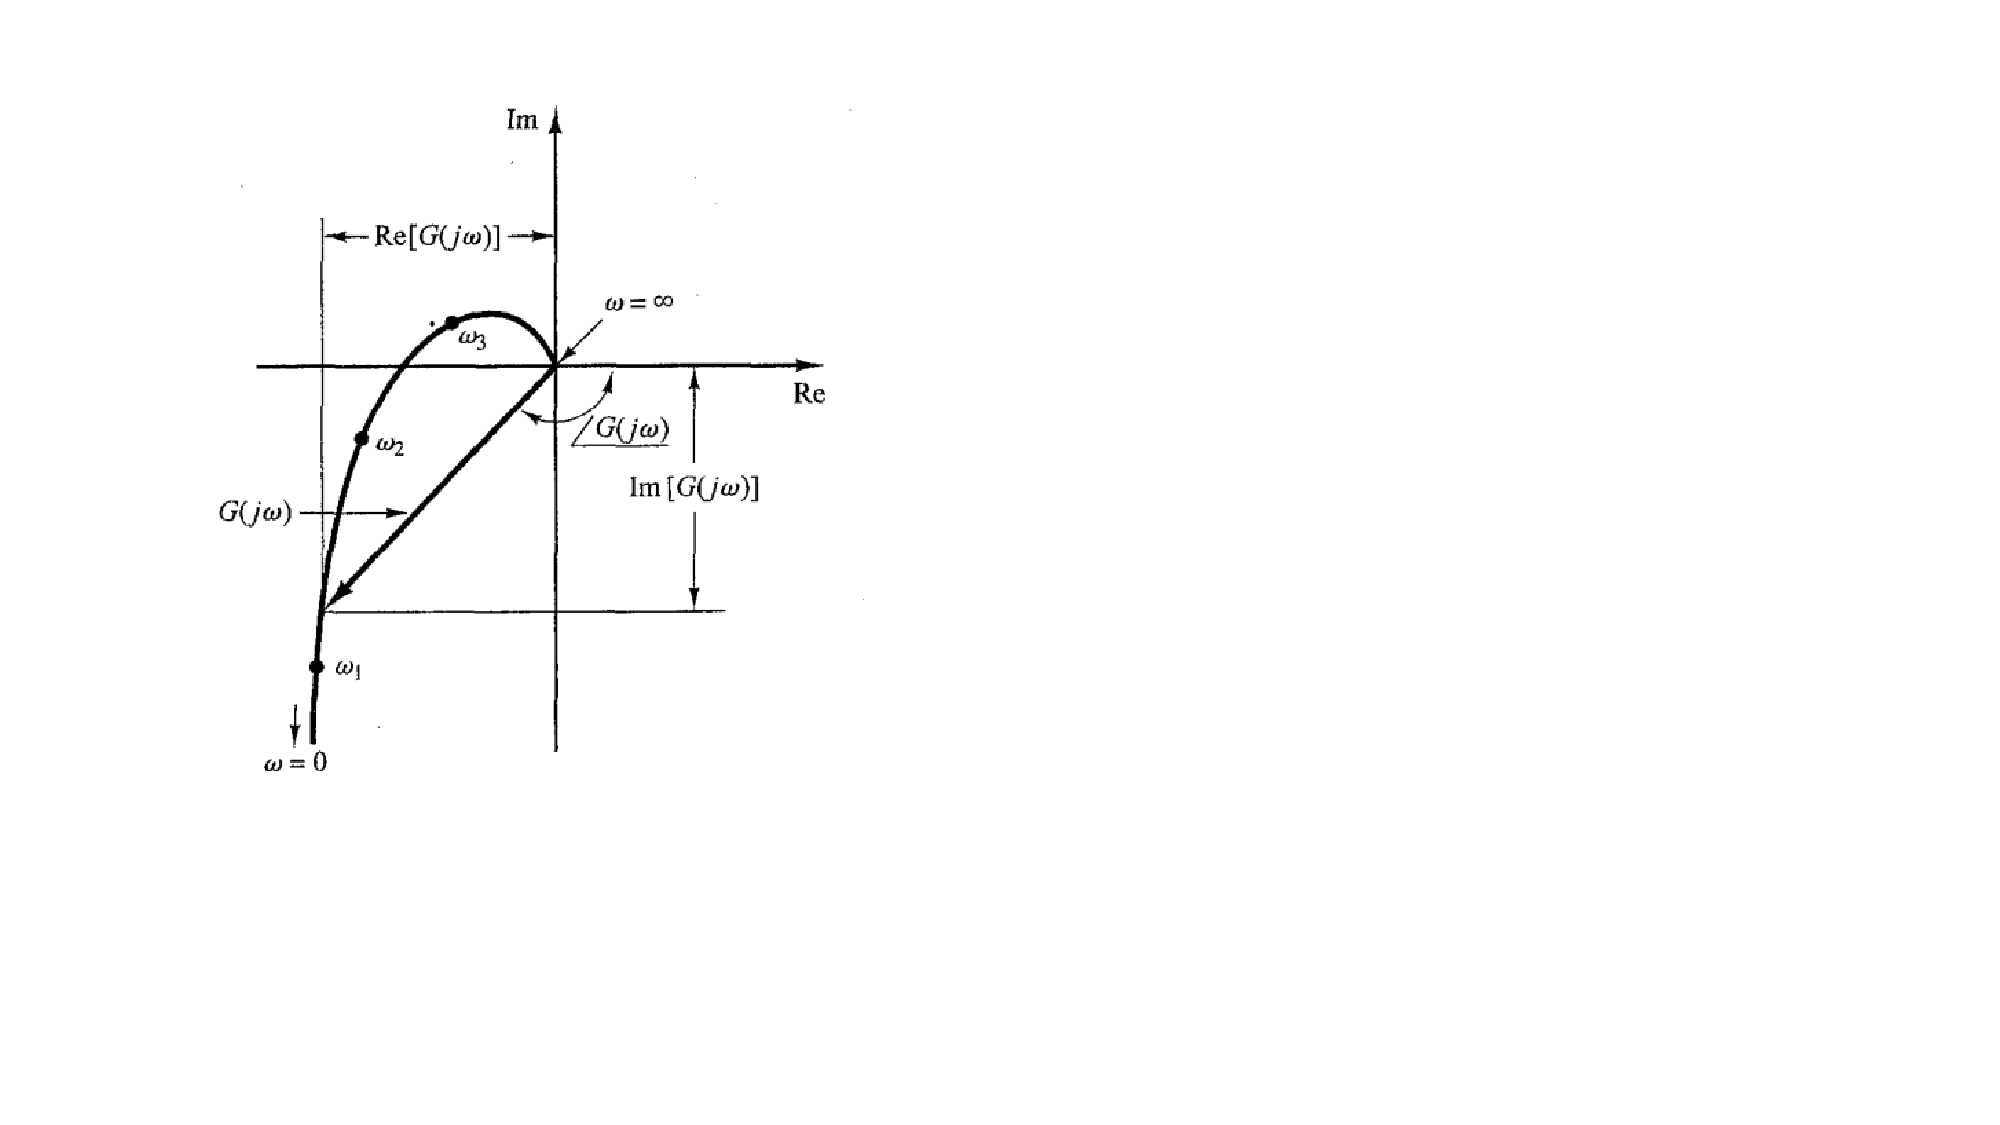
\includegraphics[scale=0.5]{NyquistPlot}



\end{frame}

\begin{frame}
\frametitle{Nyquist plot in matlab}
Similar to constructing the bode plot in Matlab, we first have to define the system using \textcolor{blue}{tf}, \textcolor{blue}{zpk} or \textcolor{blue}{ss}.\\
Then we use the command \textcolor{blue}{nyquist(sys)}.
\lstinputlisting{CreateNyquist.m}

\end{frame}

\begin{frame}
\frametitle{Bode and Nyquist plot}

\begin{columns}
\begin{column}{0.5\textwidth}
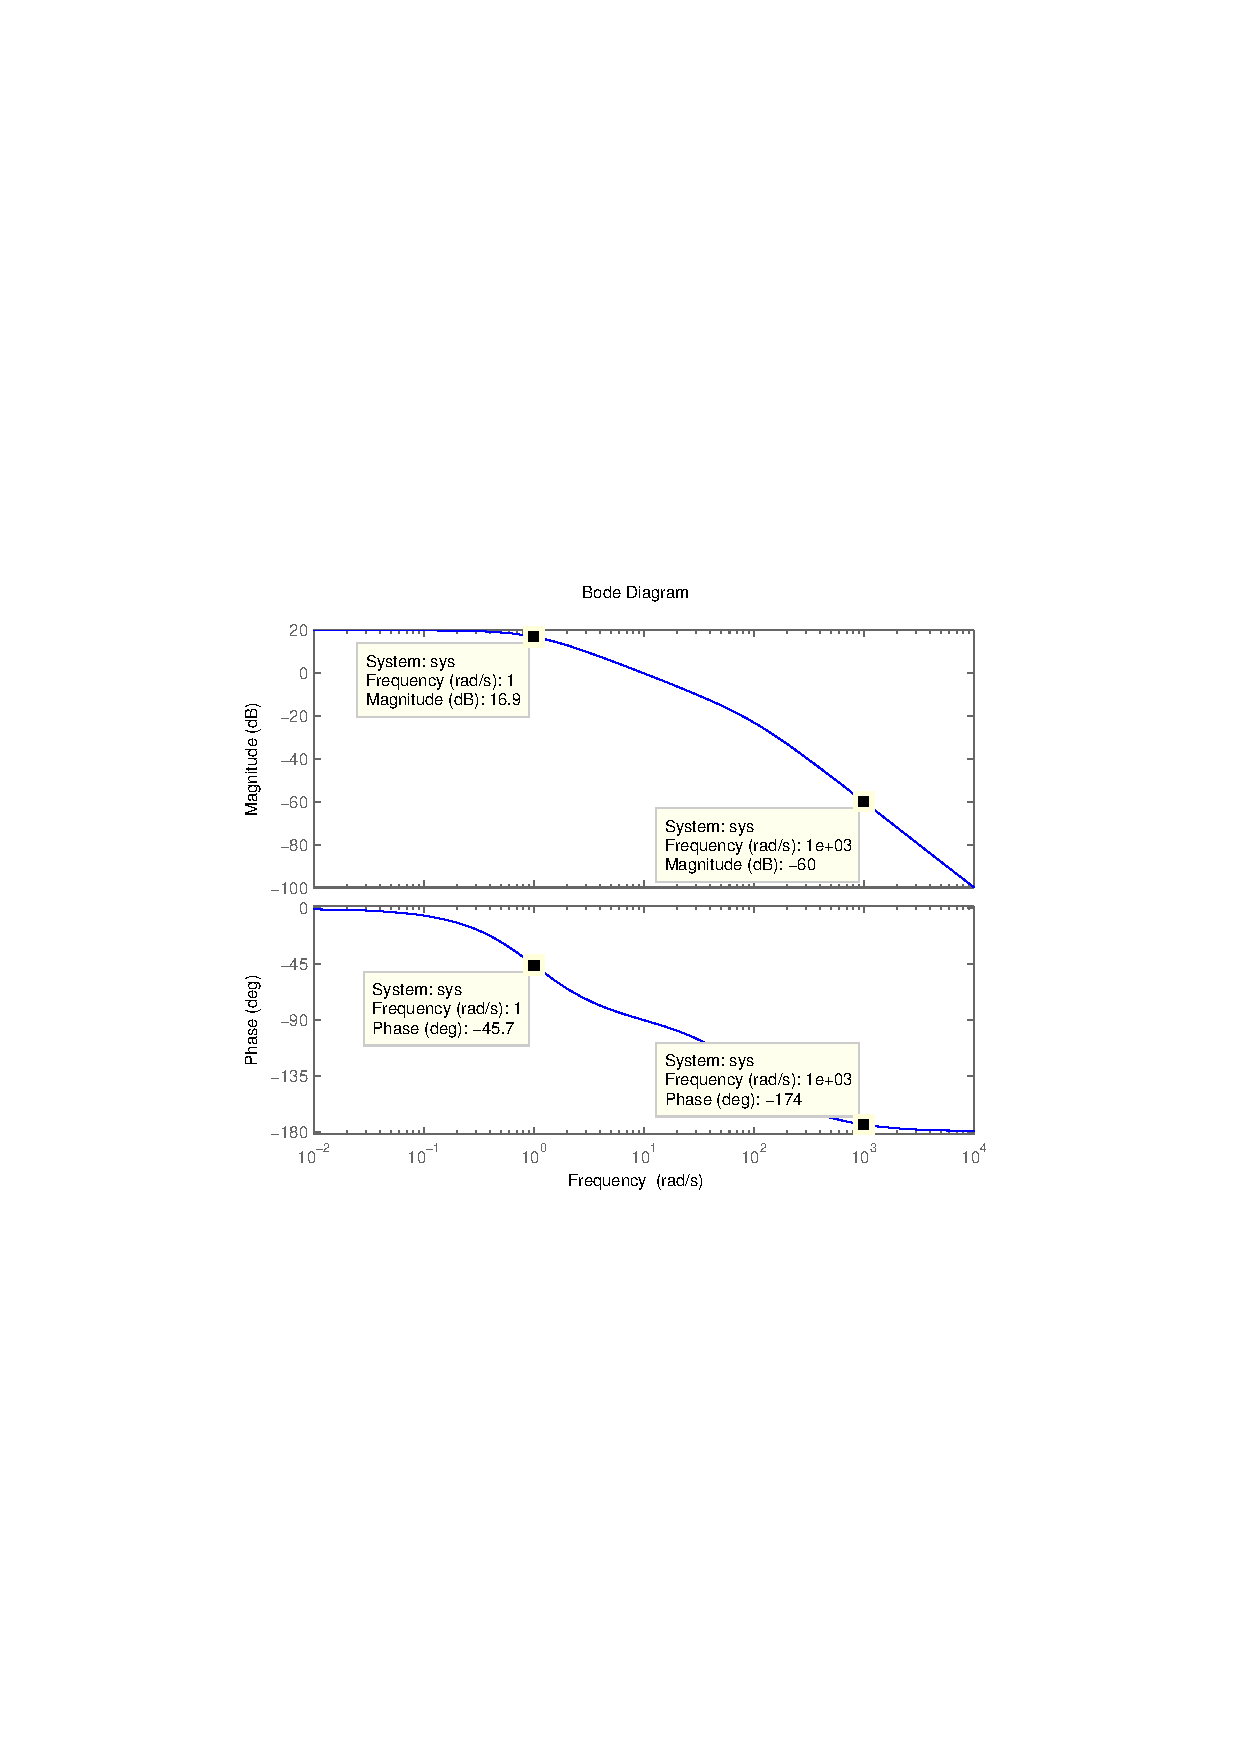
\includegraphics[scale = 0.4]{BodeVsNyquist}
\end{column}

\begin{column}{0.5\textwidth}
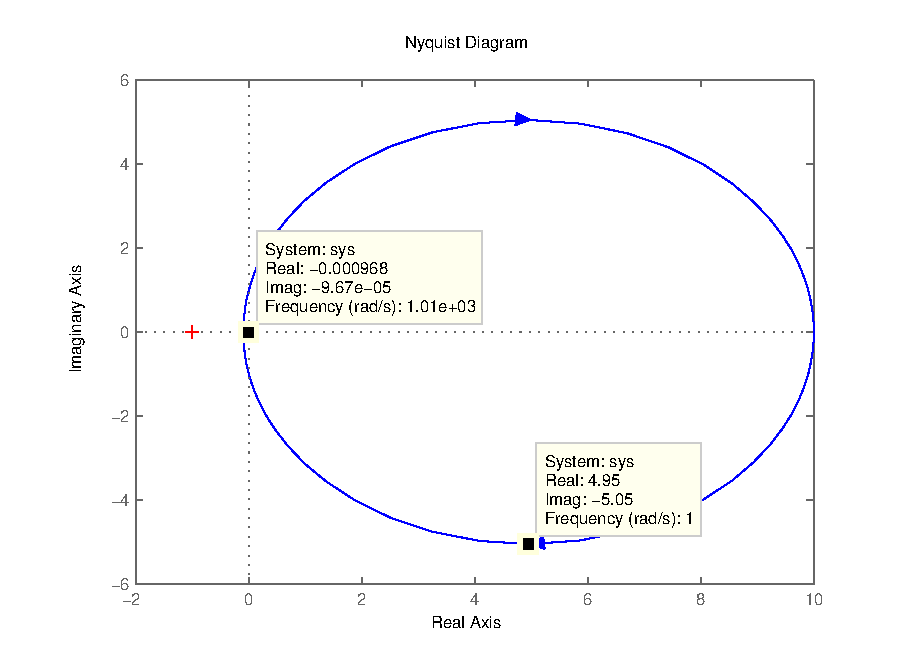
\includegraphics[scale = 0.4]{NyquistVsBode}
\end{column}
\end{columns}


\end{frame}

%\section{Conclusion}
%
%\begin{frame}
%\frametitle{Conclusion}
%
%\begin{itemize}
%\item Today we revised the basics about (constructing) the bode plot
%\item In a body plot, we can directly find the steady state response of a sinusoidal input to a linear system
%\item Bode plots will also be used in later lectures regarding controllers
%
%\end{itemize}
%
%\end{frame}


